% =====================================================================================
% Paper 1: tag-local presence guidance for NVV tags (ACL format).
% Method, experiments and figures only; the introduction is a placeholder.
% Numbers: Para/eval/superbench/GUIDANCE.md and out/ (judge qwen3.8-omni-flash, run1, seed 0).
% Code: nvv-tag-guidance (src/tagguide/contrast.py, omnivoice.py, cosyvoice.py; bench/guidance/).
% Code/method cross-check: CROSSCHECK.md in this folder.
% Build: latexmk -pdf guidance.tex
% =====================================================================================
\documentclass[11pt]{article}
\usepackage[review]{acl}
\usepackage{times}
\usepackage{latexsym}
\usepackage[T1]{fontenc}
\usepackage[utf8]{inputenc}
\usepackage{microtype}
\usepackage{inconsolata}
\usepackage{graphicx}
\usepackage{booktabs}
\usepackage{amsmath,amssymb}
\usepackage{xcolor}

\newcommand{\tg}[1]{\texttt{[#1]}}
\newcommand{\todo}[1]{\textcolor{red}{[TODO: #1]}}
\newcommand{\nt}{\textit{notag}}

\title{Tag-Local Presence Guidance for Non-Verbal Vocalization Tags in Text-to-Speech}

\author{Anonymous}

\begin{document}
\maketitle

\begin{abstract}
\todo{abstract once the story is fixed.} Draft: TTS models given an inline tag such as \tg{laughter} often leave it silent or put the sound too far away. We contrast the model with itself on the same text without the tag, only in a window of output around the tag and only while that output is still open. On the English tag-based part of NVV-SuperBench this raises F1 from 0.909 to 0.967 on OmniVoice, a masked diffusion model, at no measurable extra decoding time, and from 0.551 to 0.601 on CosyVoice~2, an autoregressive model whose window is read from its own attention. At the tag's frames the tag removes what the model would otherwise put there but spreads the probability over many tokens; the guidance concentrates it on the tokens the tag raised.
\end{abstract}

\section{Introduction}
\todo{story and contributions.}

\section{Related work}
\label{sec:related}

\paragraph{Non-verbal vocalizations in TTS.} Early work synthesizes one NVV on its own, such as laughter from pseudo-phonetic tokens \citep{xin2023laughter}. Recent models instead take inline tags in the text, learned from corpora whose transcripts mark the vocalizations \citep{borisov2025nonverbaltts,liao2025nvspeech}; CosyVoice~2 \citep{du2024cosyvoice2}, Dia \citep{nari2025dia} and OmniVoice \citep{zhu2026omnivoice} are open examples. NVV-SuperBench \citep{xue2026nvvsuperbench} asks whether the tagged NVV is heard where the tag is, and finds many tags missed or misplaced. Work so far improves tags through data and training; we change only the decoding of a trained model.

\paragraph{Guidance by contrast.} Classifier-free guidance \citep{ho2022cfg} extrapolates from the unconditional prediction towards the conditional one. It is standard in diffusion and flow-matching TTS \citep{le2023voicebox,chen2024f5tts}, is used by OmniVoice, and also works for language models \citep{sanchez2024stay}. Replacing the unconditional prediction with that of another condition steers away from it: negative and composed prompts in image diffusion \citep{liu2022composable}, an amateur model in contrastive decoding \citep{li2023contrastive}, and the same input without its context document in context-aware decoding \citep{shi2024cad}, which amplifies what the context adds to the output. Presence guidance takes this last form, with the tag as the context, and restricts it to the output the tag concerns. In TTS, guidance has been restricted to a phrase to control the accent of a code-switched span, contrasting it with another language and finding the phrase from self-attention \citep{lee2026plcg}, and adapted to autoregressive TTS for emotion, with the text's emotion in place of the dropped condition \citep{peng2025ccg}. We apply such a local contrast to NVV tags, with the tag removed as the other condition, on a masked and an autoregressive model.

\paragraph{Two families of TTS decoders.} Codec language models such as VALL-E \citep{wang2023valle} and CosyVoice~2 \citep{du2024cosyvoice2} emit discrete speech tokens one at a time, left to right. Masked generative models such as MaskGCT \citep{wang2025maskgct} and OmniVoice, following MaskGIT \citep{chang2022maskgit}, predict all masked tokens in parallel and commit the most confident first, over a fixed number of steps. Both commit a token once and never revise it, but in different orders, which decides where and when a decoding-time method can act; we use one model of each family. Section~\ref{sec:diagnosis} shows that under the confidence order a tag makes its own frames the least confident, and that presence guidance makes them confident again.

\section{Method}
\label{sec:method}
We treat the TTS model as a decoder of discrete output tokens, one per output position (and codebook). At each decoding step it gives, for every position still open, log-probabilities $c$ over the token vocabulary, conditioned on the voice prompt, the text and the tokens committed so far. It decodes from scores $\ell_0$, which are $c$ itself or a classifier-free guided form of it, and commits some of the open positions. A committed token is never revised. Section~\ref{sec:impl} gives $\ell_0$ and the commit order of the two models we use.

\subsection{Presence guidance}
\label{sec:presence}
Let $c_{\nt}$ be the model's log-probabilities for the same text with the tag removed, computed on the same output so far. Inside a window $m$ of output positions around the tag (Section~\ref{sec:window}) we add the difference between the two:
\begin{equation}
\ell = \ell_0 + \lambda\, m \odot (c - c_{\nt}),
\label{eq:presence}
\end{equation}
followed by a log-softmax, with $\lambda = 2$. As in classifier-free guidance the model is contrasted with itself, but the two inputs differ only by the tag, so the difference is what the tag asks for.

\paragraph{What the term does.} In probabilities, Eq.~\eqref{eq:presence} decodes from
\begin{equation}
p_\ell(x) \;\propto\; p_0(x)\,\Big(\frac{p_c(x)}{p_{\nt}(x)}\Big)^{\lambda}.
\label{eq:prob}
\end{equation}
By Bayes' rule $p_c(x)/p_{\nt}(x) \propto P(\text{tag}\mid x)/P(\text{no tag}\mid x)$: the ratio is the model's own detector of whether output token $x$ comes from a tagged text, and its log is the pointwise mutual information between the token and the tag. At $\lambda = 2$ a token the tag made twice as likely is multiplied by 4, a token it made less likely by less than 1, and a token it does not affect is left alone. Section~\ref{sec:diagnosis} shows why this is the right correction: at its frames the tag removes the model's default token but spreads the probability over many tokens, and Eq.~\eqref{eq:prob} concentrates it on those the tag raised.

\subsection{Localization window}
\label{sec:window}
The term acts on the output around the tag only, so the rest of the utterance, including the voice, is the model's own. Let $j_s$ be the text position where the word before the tag starts, $j_e$ the one where the word after it ends, and $A(j)$ the output position at which text position $j$ is spoken. The window is
\begin{equation}
m_i = \big[\,A(j_s) - \delta \le i < A(j_e) + \delta\,\big],
\label{eq:window}
\end{equation}
where $[\cdot]$ is 1 if the condition holds and 0 otherwise, and $\delta$ is a margin for the error of $A$. The alignment $A$ is not observed. When the output length is fixed before decoding it can be estimated from durations; when it is open, the model's attention gives its inverse, the text position each output position reads (Section~\ref{sec:impl}).

\subsection{Application schedule}
\label{sec:when}
Let $O_t$ be the output positions still open at step $t$. Only these are decoded at step $t$, and a committed token is never revised, so the term at step $t$ can change only the positions in $m \cap O_t$. We apply it with a gate $g_t \in \{0, 1\}$,
\begin{equation}
\ell^{(t)} = \ell_0^{(t)} + \lambda\, g_t\, m \odot \big(c^{(t)} - c_{\nt}^{(t)}\big),
\label{eq:gate}
\end{equation}
set to 1 while the window's positions are still open; at the other steps the pass for $c_{\nt}$ is skipped. Which steps these are depends on the commit order (Section~\ref{sec:impl}).

\section{Implementation}
\label{sec:impl}

\subsection{OmniVoice: masked generative decoding}
\label{sec:impl-omni}
OmniVoice \citep{zhu2026omnivoice} generates a fixed number $T$ of audio frames (25 per second) by iterative unmasking. Each frame holds one token per codebook. Every token starts masked; at each of 32 steps the model predicts all masked tokens and commits a scheduled number of them, the most confident first (top-token log-probability, minus a penalty growing with the codebook index, plus Gumbel noise), each committed token being the arg max of its prediction. A step runs a conditional pass on the voice prompt, the text and the frames committed so far, giving $c$, and an unconditional pass on the frames alone, giving $u$; the model decodes from the classifier-free guided scores \citep{ho2022cfg}
\begin{equation}
\ell_0 = c + \gamma\,(c-u), \qquad \gamma = 2 .
\label{eq:cfg}
\end{equation}

\paragraph{Window.} The output length is fixed before decoding, so $A$ in Eq.~\eqref{eq:window} comes from the model's own duration estimator $D$:
\begin{equation}
A(j) = T\,\frac{D(x_{<j})}{D(x)},
\label{eq:align}
\end{equation}
where $x$ is the untagged text and $x_{<j}$ its first $j$ characters. $D$ is used as OmniVoice ships it: an estimate $d$ below 50 frames (2\,s) is raised to $50\,(d/50)^{1/3}$, so a boundary within the first 2\,s of speech is placed later than its share of the text (on 62 of the 150 items, by up to 20 frames). The margin is $\delta = 0.3$\,s. Over the 150 items the window is a median of 30 frames (1.2\,s) out of 168.

\paragraph{Schedule and cost.} By step $t$ the schedule has committed about a share
\begin{equation}
\rho_t = \frac{\sigma\,\tau_t}{1 + (\sigma - 1)\,\tau_t}, \qquad \tau_t = t/32,\ \sigma = 0.1
\label{eq:rho}
\end{equation}
of the tokens: 3\% at $t = 8$, 23\% at $t = 24$. Almost the whole window is open in the first steps, so $g_t = [t \le K]$ with $K = 8$. The pass for $c_{\nt}$ runs as one more row of the same batch in those steps only; the later steps decode from Eq.~\eqref{eq:cfg}.

\subsection{CosyVoice~2: autoregressive decoding}
\label{sec:impl-cosy}
CosyVoice~2 \citep{du2024cosyvoice2} reads the prompt transcript and the text in a Qwen2 language model (LM) that emits speech tokens one at a time; a flow-matching model renders them. Its classifier-free guidance is in the flow matcher, which does not see the text, so the LM has no unconditional pass and decodes from $\ell_0 = c$ with its own repetition-aware top-$k$ sampling.

\paragraph{Window.} The output length is open, so the window is read from the model. At step $t$, let $\bar a_{t,j}$ be the conditional stream's attention from the current speech token to target-text token $j$, normalized over the target text and averaged over the heads of layers $\mathcal L = \{11, 16\}$ (0-based). The read position is
\begin{equation}
r_t = \arg\max_j\,(\kappa * \bar a_t)_j,
\label{eq:read}
\end{equation}
with $\kappa$ a three-token box filter. In these layers $r_t$ moves monotonically with $t$ (Spearman $\rho$ 0.99--1.00 on four items, against 0.08--0.45 for the mean over all layers), so it stands for $A^{-1}$, and the window of Eq.~\eqref{eq:window} becomes
\begin{equation}
m_t = \big[\,j_s - \delta \le r_{t-1} < j_e + \delta\,\big], \qquad \delta = 1\ \text{token};
\label{eq:window-cosy}
\end{equation}
the term at step $t$ uses the read position of step $t-1$.

\paragraph{Schedule and cost.} Each speech token is committed when it is emitted, so $O_t = \{t\}$ and $g_t = m_t$: the term acts at every step the window is on (a median of 25.5\% of the steps). The untagged text is a second LM stream with its own cache, fed the same sampled tokens.

\begin{figure*}[t]
  \centering
  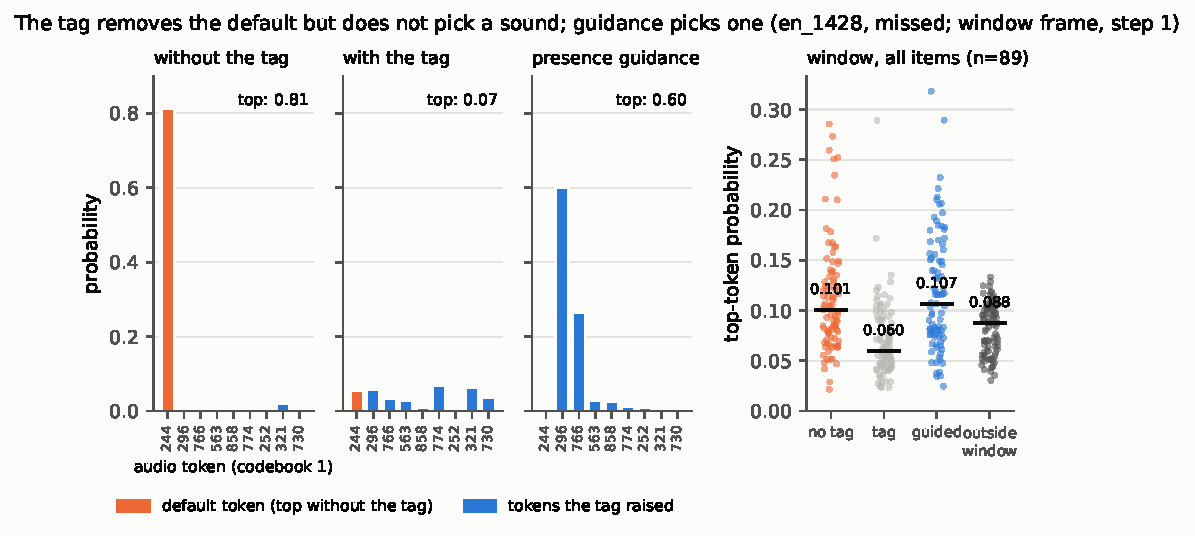
\includegraphics[width=\textwidth]{figures/fig_frame.pdf}
  \caption{Left: one frame inside the window of a missed laugh (en\_1428), first codebook, first decoding step; the model's distribution over audio tokens without the tag, with the tag, and with presence guidance (Eq.~\ref{eq:presence}). Orange: the default token (top without the tag); blue: tokens the tag raised. Right: top-token probability in the window at step 1 over the 89 items whose trace reproduces the judged clip, and outside the window.}
  \label{fig:frame}
\end{figure*}

\begin{figure*}[t]
  \centering
  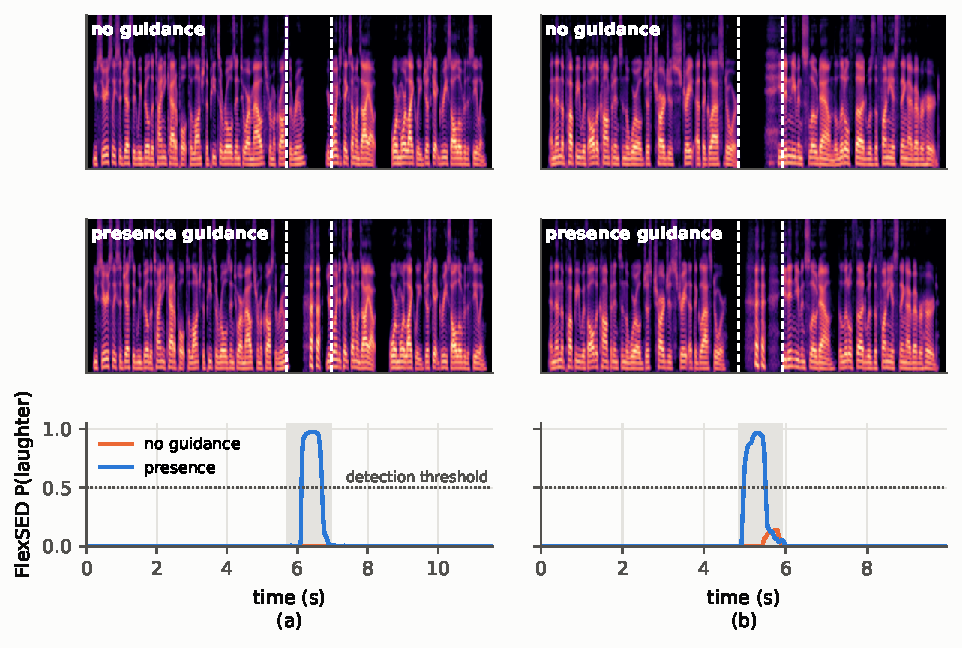
\includegraphics[width=0.85\textwidth]{figures/fig_example.pdf}
  \caption{Two laughs missed without guidance, same seed and voice: en\_1428 (no sound) and en\_1414 (a faint sound). Top two rows: mel spectrograms without and with presence guidance; dashed lines: the window. Bottom: FlexSED's laughter probability.}
  \label{fig:example}
\end{figure*}

\section{Experimental setup}
\label{sec:setup}
\paragraph{Benchmark.} The English tag-based part of NVV-SuperBench \citep{xue2026nvvsuperbench}: 2,250 sentences over 45 NVV types, each with one inline marker at a word position. A model is run on the items of the types its tags cover, with the marker replaced by its own tag: for OmniVoice \tg{laughter}, \tg{sigh}, \tg{surprise-ah}, \tg{surprise-oh} and \tg{dissatisfaction-hnn} (150 items); for CosyVoice~2 breath, laughter, cough, clucking, quick breath, hissing, sigh and lip smack (400 items, 50 per type).

\paragraph{Models and voices.} Public base checkpoints without fine-tuning: OmniVoice and CosyVoice~2 0.5B. The benchmark has no reference audio, so each item is cloned from one of two fixed English voices made once with OmniVoice's voice design, with their transcripts. Each item is synthesized once with seed 0, the same seed and voice in every setting, and all OmniVoice settings, including no guidance, run through the same decoding loop. OmniVoice's upstream inference tokenizes each tag apart from the text around it, unlike its training; we tokenize the whole text at once in every setting.

\paragraph{Judge and metrics.} An audio language model hears the clip with the text and the target type and reports whether the NVV is present and before which word. This is the benchmark's verifier with Qwen3.8-Omni-Flash \citep{qwen2025omni} in place of Gemini~2.5~Pro, which no longer accepts new users; with one run, settings compare with each other but not with the published tables. A detection within 2 words of the tag is a hit, giving precision, recall and F1, and against no guidance we count the items fixed and broken (exact sign test). Each item is a \emph{hit}, \emph{off} (target heard further away), \emph{other} (only another NVV heard) or \emph{none}. WER is from Whisper large-v3 \citep{radford2023whisper} against the untagged text, capped at 1 per clip (Whisper spells a long hiss as ``s-s-s\ldots''); SIM-o is the cosine similarity of WavLM-large \citep{chen2022wavlm} ECAPA-TDNN \citep{desplanques2020ecapa} embeddings of the clip and the voice prompt; both are compared per item (sign or Wilcoxon test). RTF is measured on one RTX~5070~Ti.

\paragraph{Settings and controls.} Presence $\lambda = 2$. Controls (OmniVoice unless stated): the same contrast on every frame (\emph{global}); in all 32 steps; and with the window replaced by an attention-derived mask \citep{lee2026plcg}.

\section{Results}
\label{sec:results}

\begin{table}[t]
  \centering
  \small
  \setlength{\tabcolsep}{4pt}
  \resizebox{\columnwidth}{!}{%
\begin{tabular}{llccccr}
    \toprule
    Model & Setting & P & R & F1 & Fix/brk ($p$) & RTF \\
    \midrule
    OmniVoice   & none     & .918 & .900 & .909 & -- & .153 \\
                & presence & .967 & .967 & \textbf{.967} & 12/2 (.013) & .153 \\
    \midrule
    CosyVoice 2 & none     & .568 & .535 & .551 & -- & 0.80 \\
                & presence & .605 & .596 & \textbf{.601} & 68/45 (.038) & 1.33 \\
    \bottomrule
  \end{tabular}}
  \caption{NVV-SuperBench, English tag-based part (OmniVoice 150 items, CosyVoice~2 400); one run of the substitute judge. Fix/brk: items hit with the setting and missed without guidance, and the reverse; $p$: exact two-sided sign test.}
  \label{tab:main}
\end{table}

\subsection{Main results}

\begin{table}[t]
  \centering
  \small
  \begin{tabular}{llrrrr}
    \toprule
    Model & Setting & Hit & Off & Other & None \\
    \midrule
    OmniVoice   & none     & 136 & 11 & 0 & 3 \\
                & presence & 146 & 4  & 0 & 0 \\
    CosyVoice 2 & none     & 213 & 113 & 43 & 31 \\
                & presence & 236 & 85  & 63 & 16 \\
    \bottomrule
  \end{tabular}
  \caption{Outcome of each item. Off: target heard more than 2 words from the tag; other: target not heard, another NVV heard; none: nothing heard.}
  \label{tab:outcomes}
\end{table}

Presence guidance raises F1 from 0.909 to 0.967 on OmniVoice (12 items fixed, 2 broken, $p = .013$) and from 0.551 to 0.601 on CosyVoice~2 (68/45, $p = .038$; Table~\ref{tab:main}). Without guidance most misses are a sound too far from the tag (\emph{off}) or no sound; OmniVoice never voices another NVV instead (Table~\ref{tab:outcomes}). Guidance reduces both (none 3$\to$0 and 31$\to$16, off 11$\to$4 and 113$\to$85). It does not choose the sound: on CosyVoice~2 \emph{other} rises from 43 to 63, mostly a hesitation \emph{hmm}.

\subsection{Diagnosis on OmniVoice}
\label{sec:diagnosis}

\begin{table}[t]
  \centering
  \small
  \begin{tabular}{lrcc}
    \toprule
    Tag & Items & KL to no tag & KL to closest tag \\
    \midrule
    laugh & 50 & 0.258 & 0.068 \\
    sigh  & 50 & 0.391 & 0.144 \\
    ah    & 16 & 0.418 & 0.075 \\
    oh    & 16 & 0.358 & 0.062 \\
    hmm   & 18 & 0.396 & 0.179 \\
    \bottomrule
  \end{tabular}
  \caption{OmniVoice: how far the prediction in the tag's window moves when the tag is removed, and when it is replaced by the closest other tag (KL, first 8 steps, mean over codebooks).}
  \label{tab:kl}
\end{table}

Removing the tag moves the prediction in the window 2--5 times more than swapping it for the closest other tag (Table~\ref{tab:kl}): the tag mainly encodes that a sound goes there. At its frames the tag removes the default token but spreads the probability (Figure~\ref{fig:frame}, left): token 244 falls from 0.81 to 0.05, and the best of the tokens the tag raised gets only 0.07. Guidance multiplies the default by $(0.05/0.81)^2 \approx 0.004$ and gives 0.60 to a raised token. Over 89 items the median top-token probability in the window at step 1 is 0.060 with the tag, against 0.101 without it ($p = 4\cdot10^{-14}$), 0.088 outside the window and 0.107 with guidance (Figure~\ref{fig:frame}, right). The tag's frames are thus the least confident in the clip, while OmniVoice commits the most confident tokens first; we expect them to be filled last, pulled towards speech or silence by the words around them (not measured). This holds for hits and misses alike (0.066 against 0.060), so it is a risk on every tagged item rather than the cause of a miss.

Figure~\ref{fig:example} shows two missed laughs: with guidance a laugh appears in the window and the speech outside it is unchanged. The laughter probability of FlexSED \citep{hai2025flexsed}, an open-vocabulary sound event detector, rises from 0 and 0.14 to 0.97; over the 100 laugh and sigh items, its median peak in the window rises from 0.002 to 0.13 ($p = 3\cdot10^{-6}$).

\subsection{Dependence on the read position}
On CosyVoice~2 the read position never reaches the tag's tokens on 98 of the 400 unguided items. On the other 302, guidance fixes 55 items and breaks 26 ($p = .0017$); on these 98, it fixes 13 and breaks 19 ($p = .38$). Where the model reads through the tag, $c$ and $c_{\nt}$ barely differ and the guided clip is only another sample.

\subsection{Window and steps}
\label{sec:window-res}

\begin{table}[t]
  \centering
  \small
  \setlength{\tabcolsep}{4pt}
  \begin{tabular}{lccc}
    \toprule
    OmniVoice & WER & SIM-o & SIM-o loss $>$0.1 \\
    \midrule
    no guidance        & 0.056 & 0.814 & -- \\
    presence, window   & 0.061 & 0.810 & 1 \\
    presence, global   & 0.061 & 0.777 & 12 \\
    \bottomrule
  \end{tabular}
  \caption{Intelligibility and speaker similarity (means over 150 items). Last column: clips whose SIM-o drops by more than 0.1 against no guidance.}
  \label{tab:quality}
\end{table}

The tag's effect is local: the no-tag KL falls to 0.21--0.32 of its in-window value within 25 frames of the window and to 0.05--0.08 beyond 50. Applying the term on every frame keeps the hits but changes the speaker (Table~\ref{tab:quality}): SIM-o falls by 0.037 (Wilcoxon $p = .001$) and 12 clips lose more than 0.1, against 0.004 ($p = .18$) and one clip with the window. The window's exact form matters less: an attention-derived mask \citep{lee2026plcg} gives F1 0.977 against 0.967 (2/3 items differ, $p = 1$). Guiding all 32 steps instead of the first 8 adds nothing (145 against 143 hits on 146 items, $p = .5$).

\subsection{Cost and side effects}
On OmniVoice the extra row runs in the first 8 steps of the same batch and the RTF is unchanged. On CosyVoice~2 the second LM stream raises it from 0.80 to 1.33. Running that stream only at steps in the window, with the tokens emitted since its last run fed as one chunk, gives the same clips up to float error (at most $4\cdot10^{-4}$ per sample on 48 items) and lowers the RTF from 1.56 to 1.08, against 0.93 without guidance (one session, slower than the main runs). On CosyVoice~2 guidance also costs some intelligibility and similarity: WER rises from 0.044 to 0.052 (higher on 84 items, lower on 42, $p < .001$) and SIM-o falls from 0.749 to 0.741 (lower on 231 of 400, $p = .002$). On OmniVoice WER is higher on 21 items and lower on 9 ($p = .043$), with the same median.

\section*{Limitations}
One seed, one run of a substitute judge, and few missed items on OmniVoice (14 of 150), so differences of a few items are trends. The diagnosis of Section~\ref{sec:diagnosis} is on OmniVoice only, and the commit order it implies is not measured. No listening test.

\bibliography{refs}

\end{document}
